\chapter{Simulation results}

The last step here, is to simulate the power train, related with all the elements inside, as battery bank, power converters, electric motor, etc.

\begin{figure}[h]
    \centering
    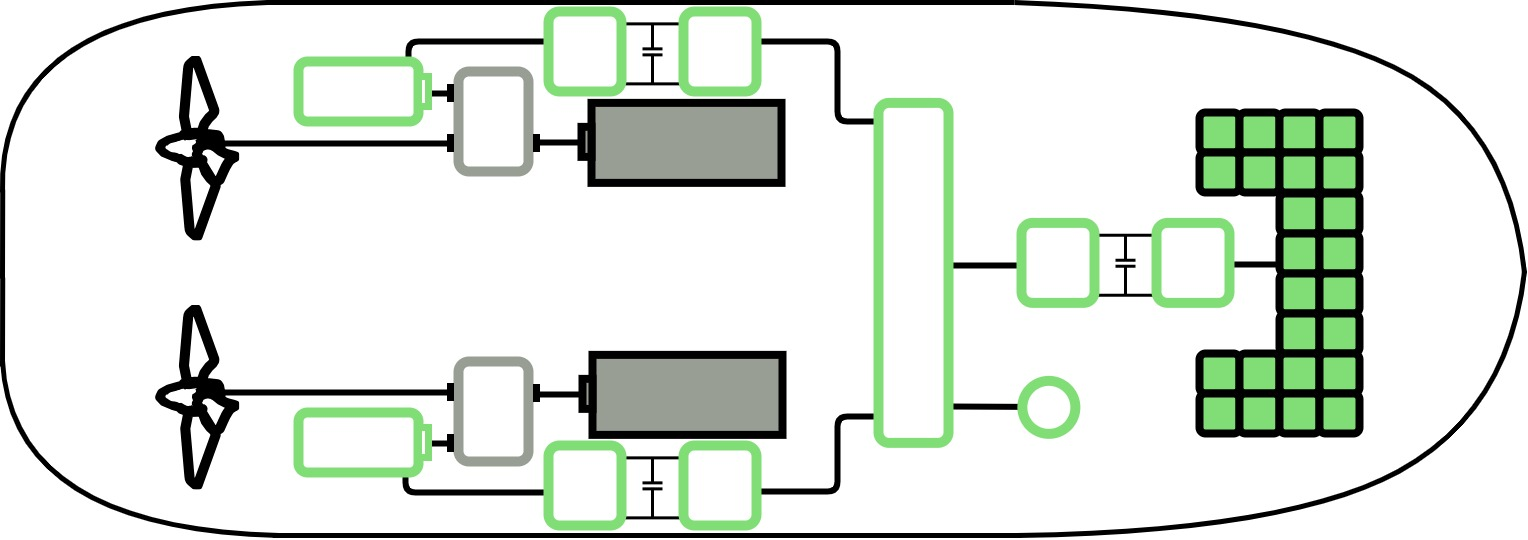
\includegraphics[width=0.75\textwidth]{images/chapter05/PowerTrain.jpg}
    \caption{PowerTrain}
    \label{PowerTrain}
\end{figure}

\section{Battery Cell}

\begin{figure}[h]
    \centering
    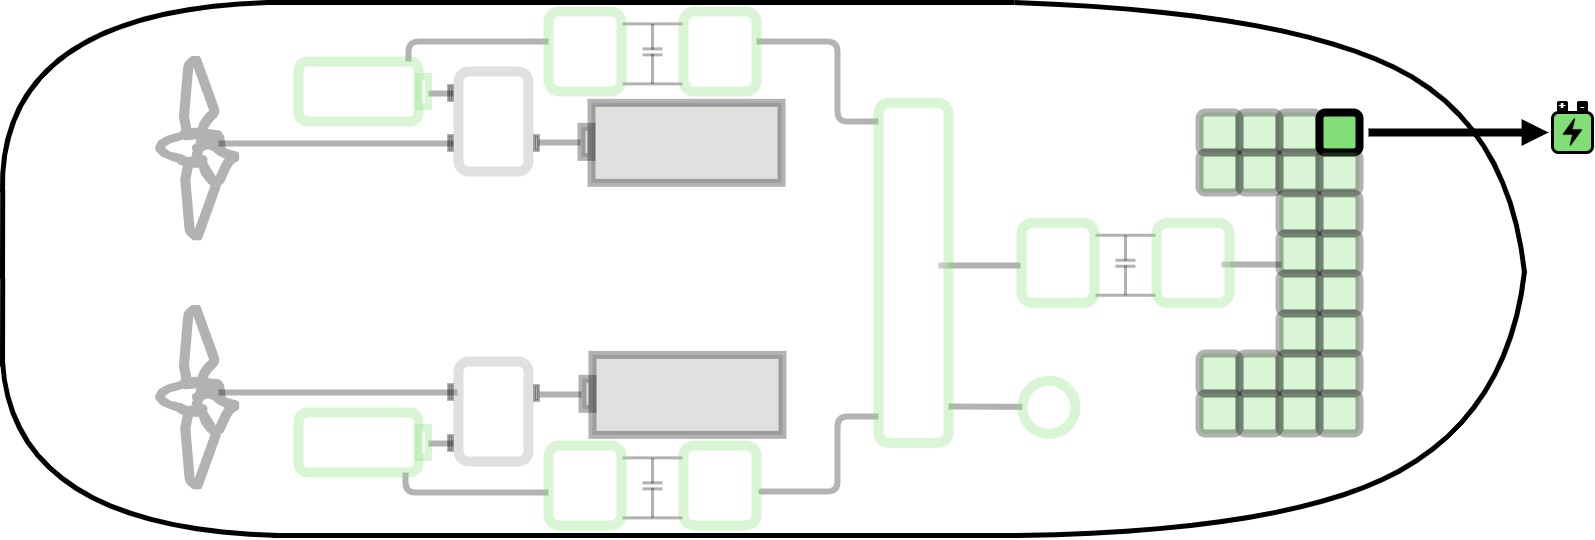
\includegraphics[width=0.75\textwidth]{images/chapter05/BattCell_scheme.jpg}
    \caption{BattCell in power train.}
    \label{BattCell}
\end{figure}

The battery bank’s design parameters are used to select a cell for electrical modeling with a Shepherd model of order 0. Technical details of the chosen cell, U27-36XP from Valence, are used to find model parameters that closely match its real discharge curve. The model shows good similarity to the actual performance, as illustrated in Fig. 12. This enables the extrapolation of results to model a battery bank and predict its behavior across various operating profiles.




\section{Battery Bank}

\begin{figure}[h]
    \centering
    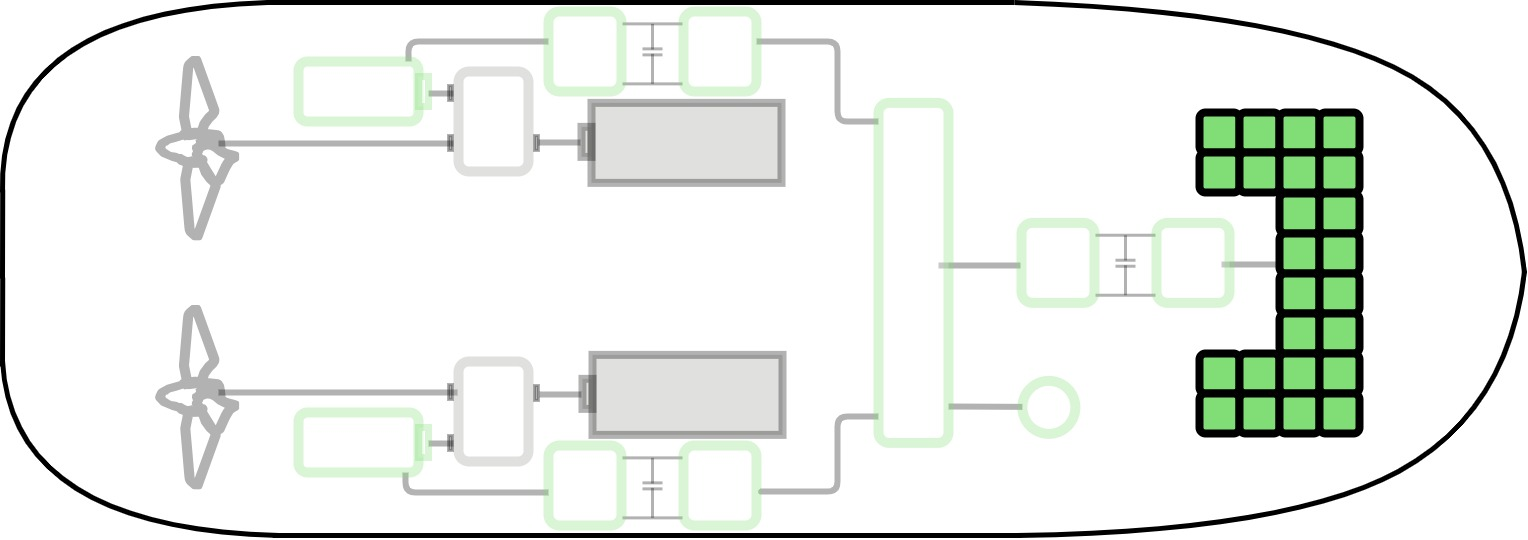
\includegraphics[width=0.75\textwidth]{images/chapter05/BattBank_scheme.jpg}
    \caption{BattBank in power train.}
    \label{BattBank}
\end{figure}

\section{Electric Motor}

\begin{figure}[h]
    \centering
    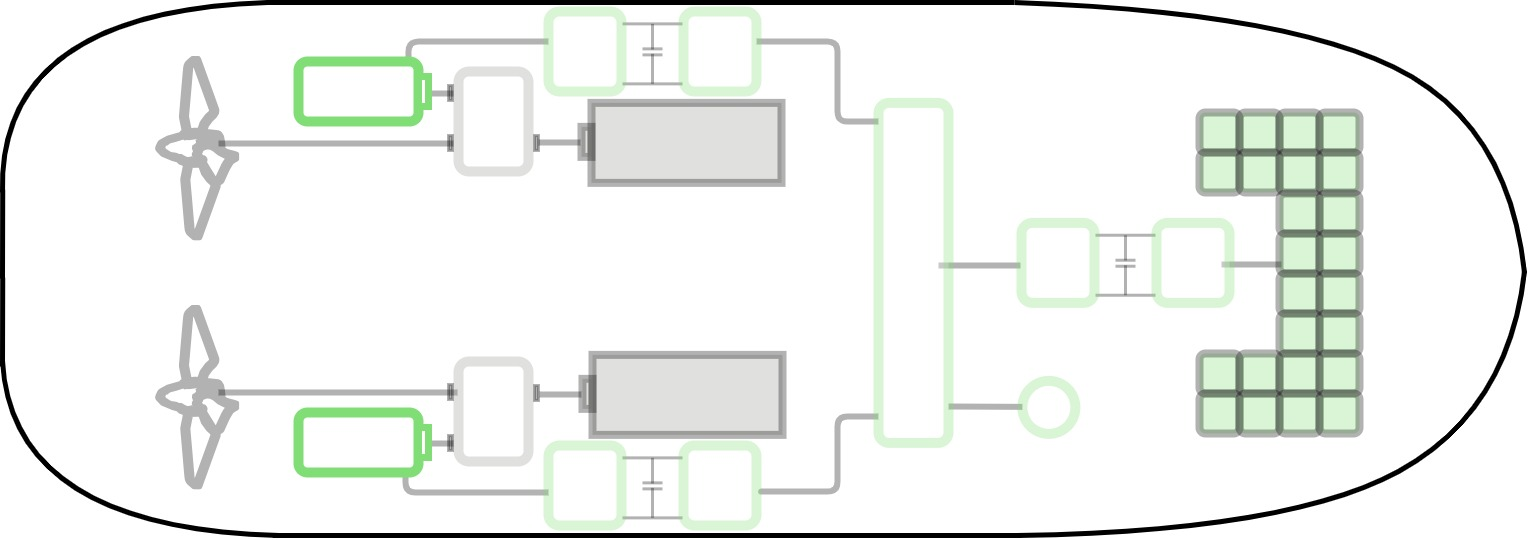
\includegraphics[width=0.75\textwidth]{images/chapter05/ElectricMotor_scheme.jpg}
    \caption{ElectricMotor in power train.}
    \label{ElectricMotor}
\end{figure}

\newpage

\section{Diesel Propulsion Engine}

\begin{figure}[!ht]
    \centering
    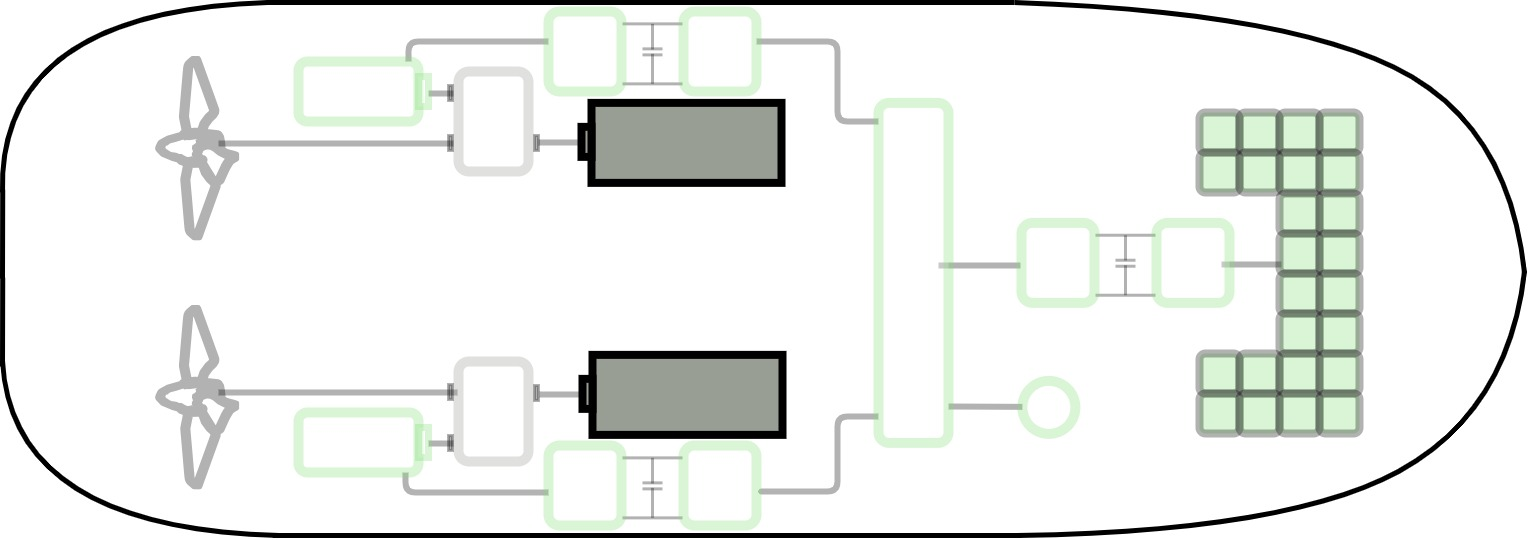
\includegraphics[width=0.75\textwidth]{images/chapter05/DieselEngine_scheme.jpg}
    \caption{Diesel Propulsion Engine in power train.}
    \label{Diesel Engine}
\end{figure}

\section{Propeller}

\begin{figure}[!ht]
    \centering
    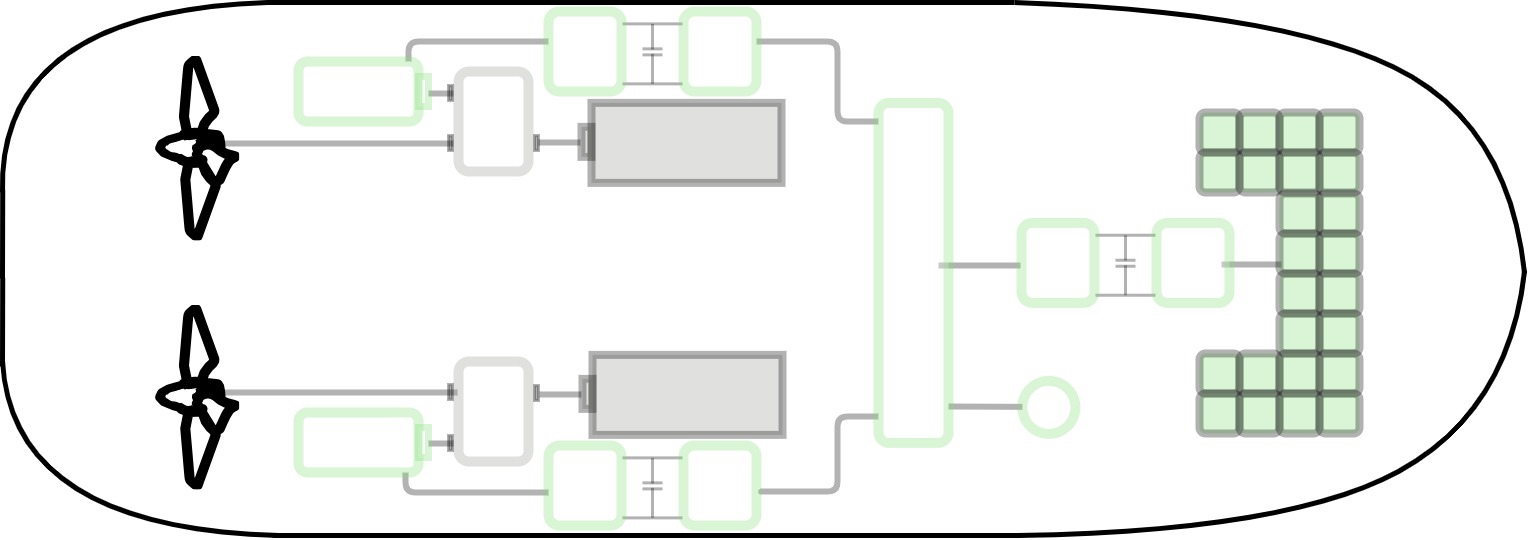
\includegraphics[width=0.75\textwidth]{images/chapter05/Propeller_scheme.jpg}
    \caption{Propeller in power train.}
    \label{Propeller}
\end{figure}

- Explicación
- Curva hélice
- Simulaciones de Potencia